\documentclass[12pt]{article}
%\usepackage[margin=1in, paperwidth=35.43in, paperheight=47.24in]{geometry}
\usepackage[a0paper, margin=1in]{geometry}
\usepackage{graphicx}
\usepackage{tikz}
\usepackage{lipsum} % Para gerar texto de exemplo
\usepackage{anyfontsize}
\usepackage{caption}
% Configura para porguês do Brasil
\usepackage[T1]{fontenc}
\usepackage[utf8]{inputenc}
\usepackage[portuguese]{babel}
\usepackage{parskip}
\usepackage{ragged2e}

% Configura a font padrão para Source Code Pro
%\renewcommand*\familydefault{\ttdefault}
% comando \textbf é Source Code Pro negrito
%\renewcommand{\bfdefault}{sb}

\begin{document}
\pagestyle{empty} % Remove número de página e cabeçalhos

% Título, autores, e filiação
\begin{center}
    \textbf{
    {\fontsize{50}{60}\selectfont Da Terra ao Código: Integrando Dados Geológicos\\
                                        à Inteligencia Computacional}\\[20mm] % Tamanho do título
    {\fontsize{40}{48}\selectfont Gabriel Góes Rocha de Lima}\\[5mm] % Tamanho dos autores
    {\fontsize{35}{42}\selectfont Universidade de São Paulo}\\[20mm] % Tamanho da filiação
    \rule{1\textwidth}{0.4pt} % Linha horizontal
    }
\end{center}

% Inserir logos
\begin{tikzpicture}[remember picture,overlay]
    \node[anchor=north west, yshift=-1.5cm, xshift=2cm] at (current page.north west) 
        {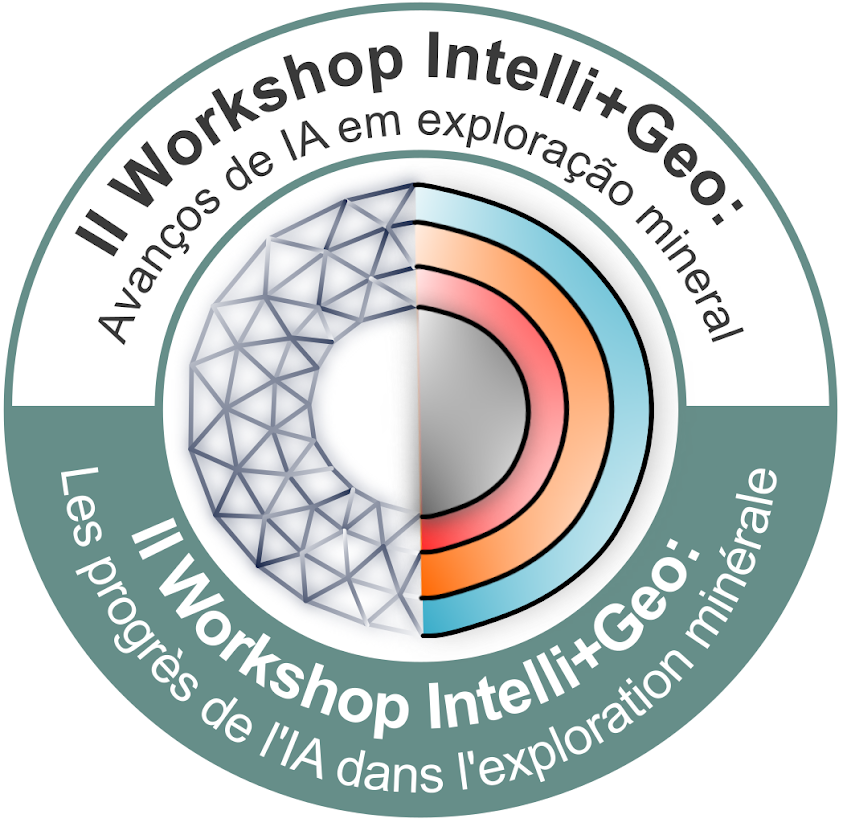
\includegraphics[width=10cm]{../resumos/logo.png}}; % Ajuste o caminho e tamanho
    \node[anchor=north east, yshift=-7.8cm, xshift=-1.8cm] at (current page.north east) 
        {
\includegraphics[width=15cm]{./IGC.png}}; % Ajuste o caminho e tamanho
    \node[anchor=north east, yshift=-1.8cm, xshift=-5cm] at (current page.north east) 
        {
\includegraphics[width=10cm]{./INRS.png}}; % Ajuste o caminho e tamanho
\end{tikzpicture}

%%%%%%%%%%%%%%%%%%%%%%%%%%%%%%%%%%%%%%%%%%%%%%%%%%%%%%%%%%%%%%%%%%%%%%%%%%%%%%%
% Introdução
\begin{minipage}[t]{\textwidth}
\chapter{Introdução}
\section{Considerações Iniciais}
\par{A grafita, um mineral de relevância crescente no panorama tecnológico e industrial, destaca-se por suas propriedades únicas e aplicações versáteis, desde o desenvolvimento de nanomateriais, como o grafeno, até seu uso em produtos industriais diversos. Este projeto de pesquisa foca na exploração de jazidas de grafita utilizando técnicas avançadas de aprendizado de máquina e sensoriamento remoto, concentrando-se no sistema de nappes de Socorro-Guaxupé.}

\par{Exploramos como os métodos geofísicos, em conjunto com o processamento de dados aerogeofísicos, podem ser utilizados para identificar padrões associados à mineralização de grafita. O objetivo é desenvolver um modelo preditivo robusto que melhore a eficiência da prospecção mineral e a gestão dos recursos naturais.}

\par{Esta pesquisa se insere em um contexto onde a demanda por grafita está em ascensão devido às suas aplicações em tecnologias emergentes. A grafita é amplamente distribuída em diversos tipos de rochas, mas a identificação de depósitos economicamente viáveis é um desafio que requer abordagens inovadoras. A integração de dados geofísicos com técnicas de aprendizado de máquina apresenta uma oportunidade única para abordar essa questão, potencializando a identificação de áreas promissoras para exploração mineral.}

\begin{minipage}[t]{0.45\textwidth}
% Fundamentação Teórica
% INTRODUÇÃO
% - Breve introdução ao contexto e à importância da integração de dados geológicos
%   com inteligência computacional.
% - Apresente o problema que o projeto visa resolver.

\setlength{\fboxsep}{1cm}% Controla o espaçamento interno do fbox
\fbox{% Cria um box ao redor do texto
    \parbox{\textwidth}{% Permite o controle de parágrafo dentro do fbox
        \setlength{\parindent}{1.5cm} % Define a identação dos parágrafos
        \fontsize{30}{36}\selectfont % Ajusta o tamanho da fonte e o espaçamento de linha
        \textbf{Fundamentação Teórica}\\
\par{
    A coleta, armazenamento e gestão eficiente de dados geológicos formam a espinha dorsal do nosso projeto. Utilizando o PostgreSQL com a extensão PostGIS, estabelecemos uma infraestrutura robusta capaz de lidar com a complexidade e o volume crescente de dados geoespaciais. Esta infraestrutura não só permite o armazenamento detalhado de informações geológicas, mas também oferece ferramentas poderosas para sua manipulação e análise. A capacidade de realizar consultas espaciais complexas e manipular dados geográficos em tempo real é fundamental para a agilidade e precisão das análises subsequentes por modelos de IA.
}\\

\par{
    Integrando a essencial infraestrutura de dados proporcionada pelo PostgreSQL e PostGIS com a articulação sistemática de folhas cartográficas, o projeto "Da Terra ao Código" alavanca uma automação avançada no processo de predição para a exploração mineral e mapeamento geológico. Esta abordagem não só facilita o armazenamento e análise detalhada de vastos conjuntos de dados geoespaciais, mas também otimiza a geração de mapas litológicos preditivos. A implementação de folhas cartográficas no fluxo de trabalho permite a sistematização e padronização dos dados de entrada do modelo, assim como facilita as operações de requisição de dados. Esta sinergia entre a robusta gestão de dados e a integração de folhas cartográficas constitui a base para um avanço significativo na precisão e eficiência na produção de mapas litológicos preditivos para auxiliar o mapeamento geológico, assim como na produção de mapas de potencial mineral preditivos (MPM).
}\\

        \centering
        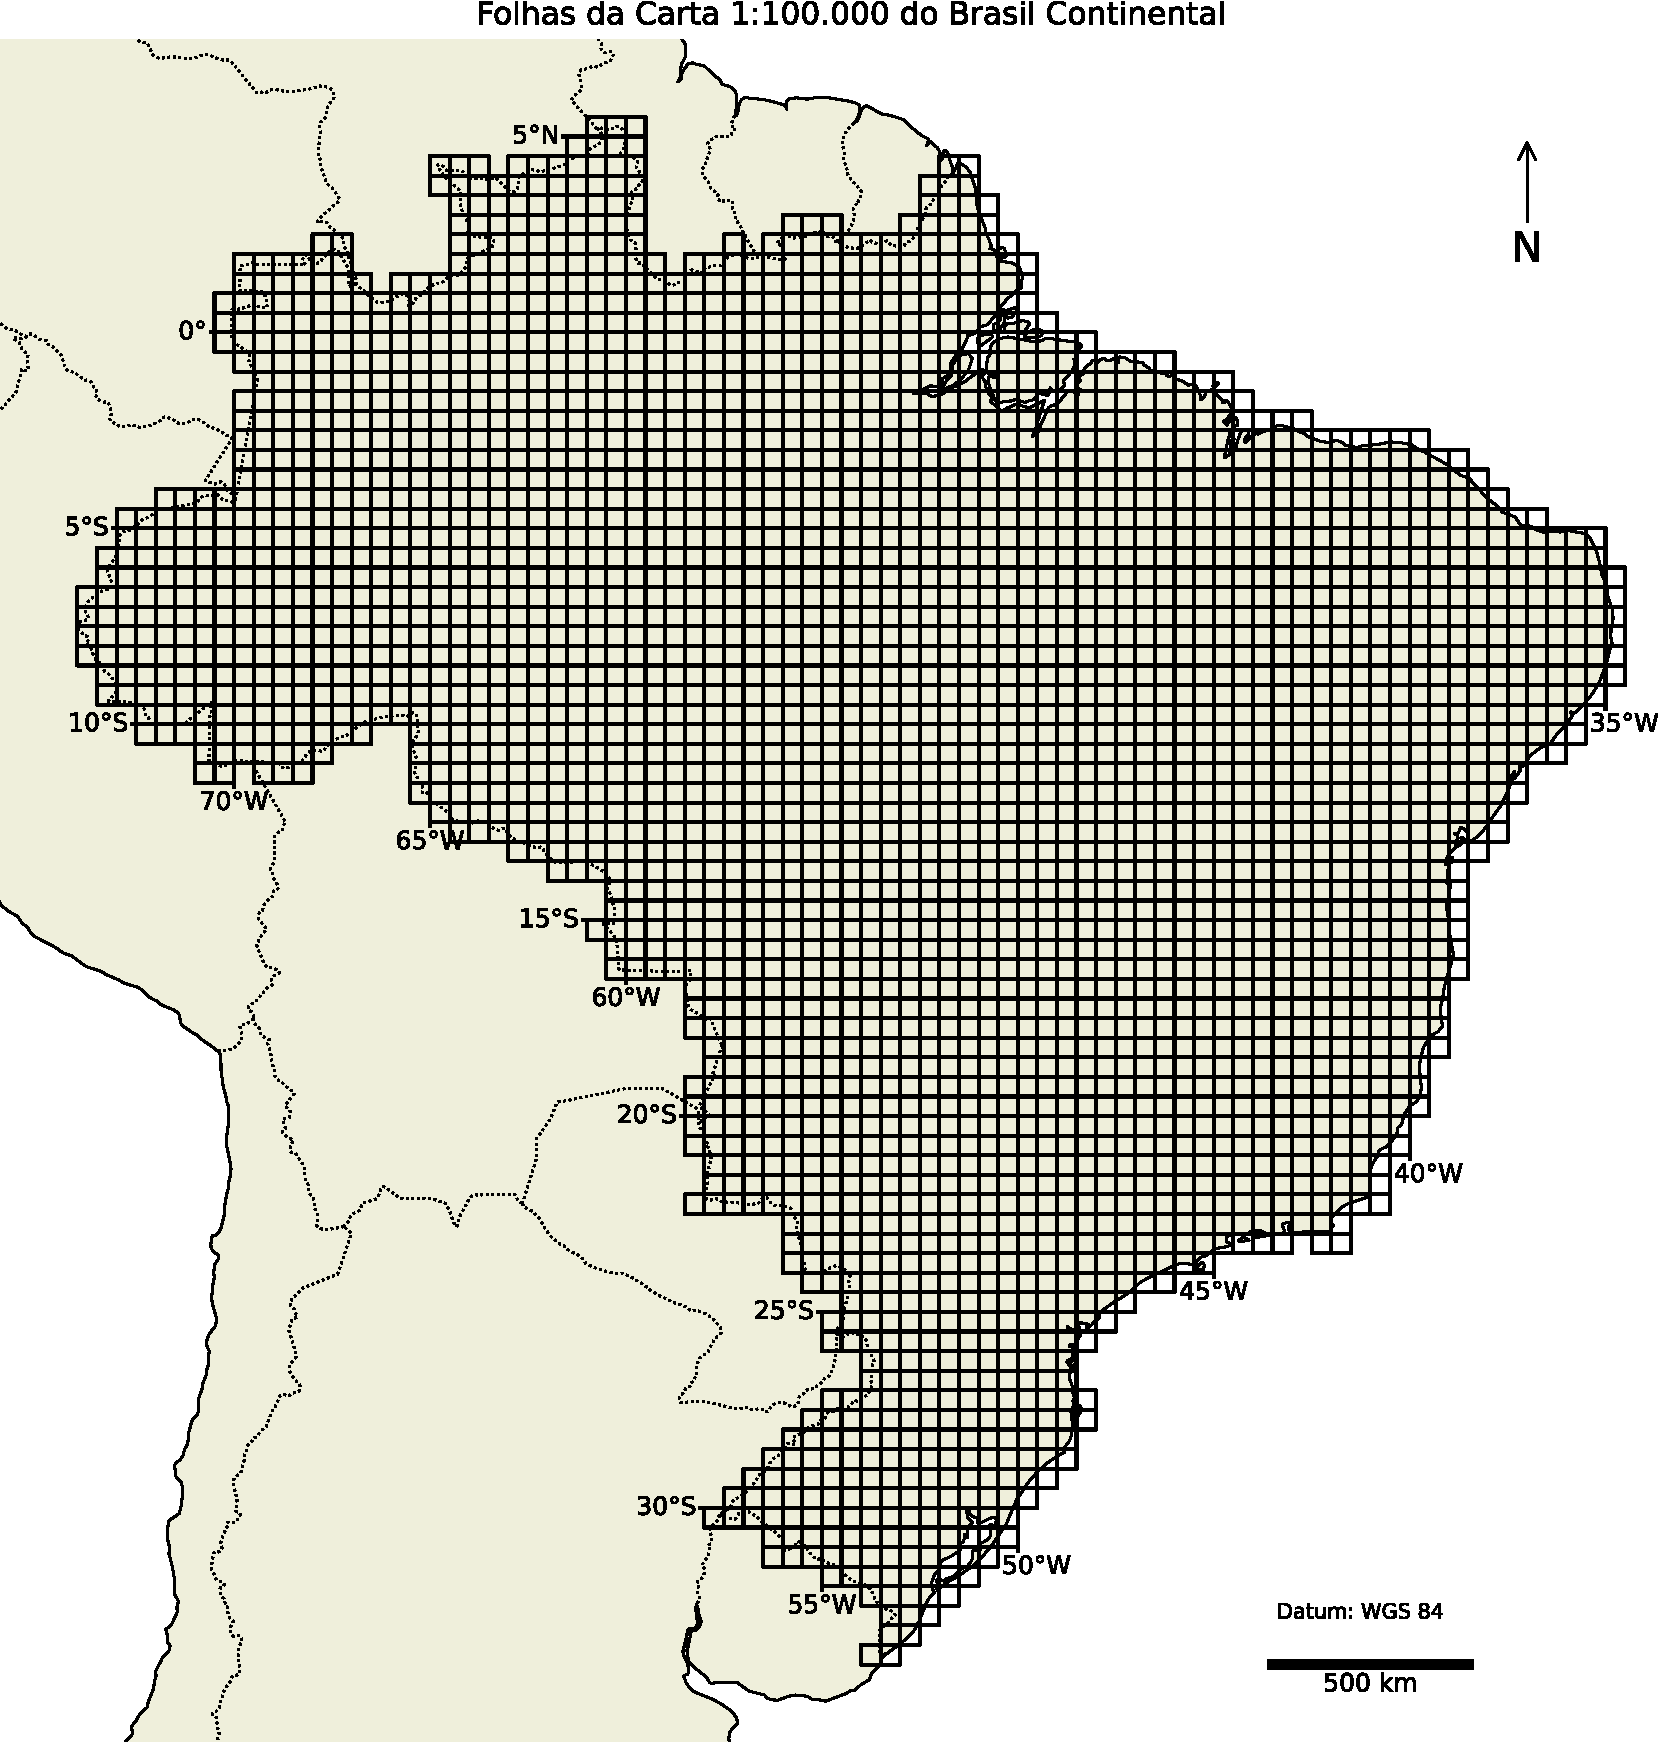
\includegraphics[width=0.9\textwidth]{../../images/100k_brasilcont.pdf}
        % Caption da imagem, legenda da figura centralizada abaixo da figura.
        \\[5mm]
        \captionof{figure}{\textbf{Representação da articulação sistemática das folhas da carta de escala 1:100.000 do Brasil continental.}}
\\[10mm]
        \justifying
        \setlength{\parindent}{1.5cm} % Define a identação dos parágrafos
\par{
    A utilização do PostgreSQL com a extensão PostGIS transforma radicalmente a gestão de dados geológicos para além das capacidades limitadas de arquivos CSV em diretórios locais. Este sistema avançado de gerenciamento de banco de dados relacional supera as abordagens convencionais ao habilitar consultas espaciais complexas e análises geoespaciais diretas, otimizando assim a integração e análise de dados para modelos de IA. Além disso, suas funcionalidades de indexação espacial e otimização de consultas garantem desempenho superior em operações de dados volumosos, enquanto mecanismos robustos de controle de acesso asseguram a integridade e a segurança dos dados. Em resumo, a escolha por PostgreSQL e PostGIS é fundamental para a eficiência, escalabilidade e precisão na exploração de dados geológicos, marcando um novo padrão em análises preditivas e no mapeamento geológico.
}
    }% fecha parbox
}% fecha fbox

\end{minipage}
% Espaço entre as colunas com o tamanho de 0.05 da largura do texto
\hspace{0.05\textwidth}
\begin{minipage}[t]{0.45\textwidth}
% Metodologia
\vspace{-41.5cm}
% METODOLOGIA
\setlength{\fboxsep}{1cm}% Espaçamento interno do fbox
\fbox{% Cria um box ao redor do texto
    \parbox{\textwidth}{% Permite o controle de parágrafo dentro do fbox
        \setlength{\parindent}{1.5cm} % Define a identação dos parágrafos
        \fontsize{30}{36}\selectfont % Ajusta o tamanho da fonte e o espaçamento de linha
        \textbf{Metodologia}\\

\par{
    A integração de dados geológicos com modelos de IA é refinada pela sistematização proporcionada pela articulação de folhas de carta. Esta sistematização não só garante a consistência e precisão na organização dos dados, mas também otimiza o processo de alimentação dos modelos de IA. As folhas de carta servem como uma estrutura base que guia a coleta de dados, garantindo que cada informação geológica inserida no banco de dados PostgreSQL/PostGIS esteja bem organizada e pronta para análise.
}\\
\par{
    O uso dessa metodologia permite uma abordagem dinâmica e iterativa para a geração de mapas litológicos preditivos. Com a estruturação dos dados facilitada pelas folhas de carta, os modelos de IA podem ser aplicados de maneira mais eficiente, proporcionando análises preditivas mais precisas. A validação dessas predições por especialistas e a reincorporação de dados validados ao banco promovem um ciclo contínuo de aprimoramento, destacando a importância da articulação de folhas de carta não apenas para a automação, mas também para a evolução constante do projeto.
}\\

    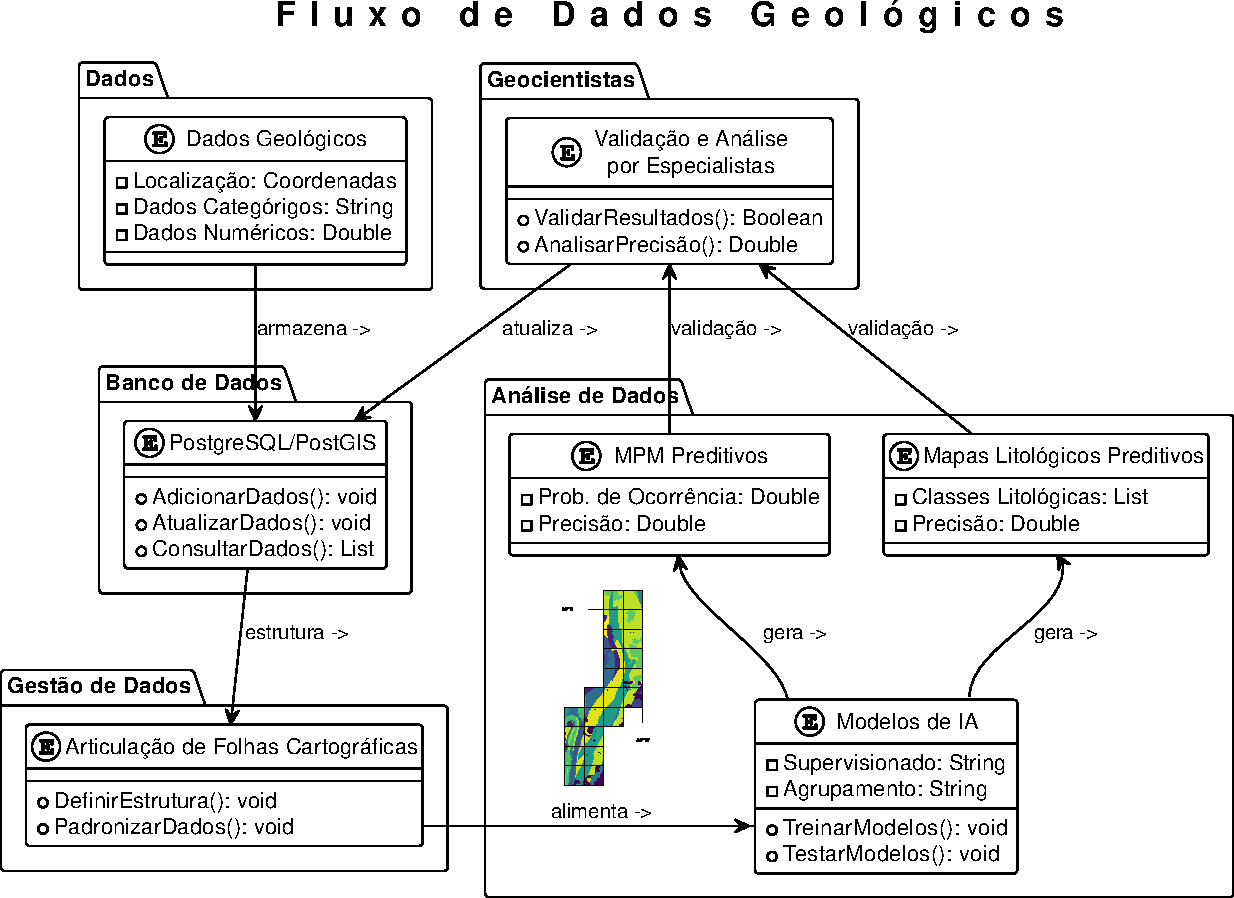
\includegraphics[width=0.9\textwidth]{../imgs/PreditorTerraa.pdf}
    \captionof{figure}{\textbf{Diagrama simplificado do fluxo de dados entre as etapas de armazenamento, estruturação, análise e validação.}}

    \vspace{1.0cm}
    \justifying
    \setlength{\parindent}{1.5cm} % Define a identação dos parágrafos
    } % Fecha o parbox
} % Fecha o fbox

\\[10mm]
% Resultados Obtidos
% RESULTADOS
\setlength{\fboxsep}{1cm}% Espaçamento interno do fbox
\fbox{% Cria um box ao redor do texto
    \parbox{\textwidth}{% Permite o controle de parágrafo dentro do fbox
        \setlength{\parindent}{1.5cm} % Define a identação dos parágrafos
        \fontsize{30}{36}\selectfont % Ajusta o tamanho da fonte e o espaçamento de linha
        \textbf{Resultados esperados}\\

\par{
    Com a implementação deste projeto, esperamos demonstrar a eficácia desta integração na produção de mapas litológicos preditivos e MPM preditivos. Através da articulação de folhas de carta e a utilização do PostgreSQL/PostGIS, antecipamos uma melhoria significativa na gestão e análise de dados geoespaciais. Este pôster visa destacar o potencial dessa metodologia integrada para transformar as práticas de mapeamento geológico e exploração mineral. Esperamos demonstrar como uma base de dados robusta, construída sobre PostgreSQL e PostGIS, pode ser integrada a modelos de inteligência artificial para criar um sistema automatizado de predição de litologias aflorantes. Este sistema não só otimiza a interpretação de dados geológicos complexos, mas também promove uma abordagem inovadora no mapeamento geológico. 
    }
} % Fecha o parbox
} % Fecha o fbox

\\[10mm]
% Conclusão e Impacto
% Conclusão
\setlength{\fboxsep}{1cm}% Espaçamento interno do fbox
\fbox{% Cria um box ao redor do texto
    \parbox{\textwidth}{% Permite o controle de parágrafo dentro do fbox
        \setlength{\parindent}{1.5cm} % Define a identação dos parágrafos
        \fontsize{30}{36}\selectfont % Ajusta o tamanho da fonte e o espaçamento de linha
        \textbf{Conclusão}\\

\par{
    O desenvolvimento deste projeto evidencia a importância da sinergia entre dados geológicos e inteligência artificial, apresentando um protótipo promissor que aguarda validação em ambientes de supercomputação. Esperamos que a divulgação desta iniciativa inspire a colaboração, não apenas para refinamento e ampliação do modelo existente, mas também para explorar seu pleno potencial em análises preditivas avançadas de mapeamento geológico. 
}\\

} % Fecha o parbox
} % Fecha o fbox

\end{minipage}
\end{minipage}
\vfill
%%%%%%%%%%%%%%%%%%%%%%%%%%%%%%%%%%%%%%%%%%%%%%%%%%%%%%%%%%%%%%%%%%%%%%%%%%%%%%%

% Linha horizontau como footer antes das informações adicionais
\begin{tikzpicture}[remember picture,overlay]
% desenhe uma linha horizontal com textwidth de comprimento e 10cm acima do sul da página
%     \draw (current page.south west) ++(2,10cm) -- ++(\textwidth,0);
    \node[anchor=center, yshift=8.5cm] at (current page.south) 
        {\noindent\rule{\textwidth}{2pt}};
\end{tikzpicture}

% Informações adicionais no rodapé
\begin{tikzpicture}[remember picture,overlay]
    \node[anchor=south west, yshift=7cm, xshift=-30cm] at (current page.south) 
        {\fontsize{20}{26}\selectfont \textbf{Referências}: Karianne J. Bergen et al. ,Machine learning for data-driven discovery in solid Earth geoscience.Science363,eaau0323(2019).DOI:10.1126/science.aau0323};
    \node[anchor=south west, yshift=4.5cm, xshift=-30cm] at (current page.south) 
        {\fontsize{40}{46}\selectfont acesse os links ou entre em cotato.};
    \node[anchor=south west, yshift=0.2cm, xshift=-39cm] at (current page.south) 
        {
\includegraphics[width=8cm]{./qrcode_github.com.png}}; % Ajuste o caminho e tamanho
    \node[anchor=south west, yshift=2.5cm, xshift=-30cm] at (current page.south) 
        {\fontsize{40}{46}\selectfont correio eletrônico: \textbf{gabrielgoes@usp.br}}; % Ajuste conforme necessário
    \node[anchor=south west, yshift=1cm, xshift=-30cm] at (current page.south) 
        {\fontsize{40}{46}\selectfont \textbf{www.github.com/Gabriel-Goes/mapeamento\_litologico\_preditivo}};
    \node[anchor=south east, yshift=0cm, xshift=45cm] at (current page.south) 
        {
\includegraphics[width=25cm]{./IGC.png}}; % Ajuste o caminho e tamanho

\end{tikzpicture}

\end{document}
